\chapter{High-Level System Design}
This section covers the high-level system design and the individual components.

\section{Bundle Identifier}
Each bundle has its bundle identifier, which is used by the Bundle Client (client henceforth) when requesting bundles from the Bundle Transport (transport henceforth) and by the Bundle Server (server henceforth) to keep track of the bundles it has received. 
Each Bundle ID consists of the client’s ID along with a counter. The counter is generated by the sender, so when the client sends a bundle to the server (upstream), it will increment its sending counter, and similarly, when the server sends a bundle to the client (downstream), it will increment its sending counter. While there may seem to be a correlation between the two counter-values, they are entirely independent of each other as they are used for different purposes.

In the upstream direction, the server uses the counters to keep track of the order of the bundles when they are received out of order or lost. The client, therefore, generates counters incrementally, allowing the server. In the downstream direction, the client uses the counters to request bundles from the transport. The server, therefore, generates the counter values such that they are the same as the values the client requests from the transport. This synchronization is maintained using the counter value and a window as explained in the Window section.

The counter is 8 Bytes and is added either before or after the Client ID based on the direction of the bundle. In the upstream direction, the counter is the 8 Most Significant Bytes (MSB) in the Bundle ID; in the downstream direction, it is the 8 Least Significant Bytes (LSB) as shown in Figures 2a and 2b respectively.

\begin{figure}[ht!]
\centering
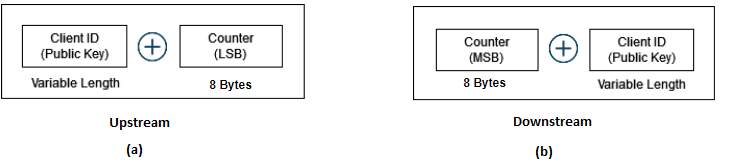
\includegraphics[width= 150mm]{./images/BundleID.png}
\caption{Bundle ID Generation}
\end{figure}

The Bundle ID will be exposed to the transport; it must therefore be encrypted to protect the client’s bundles from being identified. As we have the server’s public key, we can generate a Diffie Helman (DH) shared secret and use this as the shared secret for AES to encrypt the Bundle ID. The encrypted blob can then be sent to the transport. On the server end, it will receive the client’s public key along with the bundle. It can now generate the same shared secret and decrypt the Bundle ID. The counter value can then be obtained using appropriate bitmasks. 


\begin{figure}[ht!]
\centering
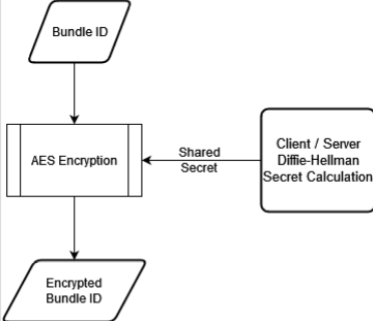
\includegraphics[width= 70mm]{./images/BundleID_Encryption.png}
\caption{Bundle ID Encryption}
\end{figure}

\section{Window}
A window is maintained at the client and server of the same size (10 by default) to provide synchronization between them when transporting bundles. The server-side window is used to keep track of the bundles sent to the client and to make sure it does not send more bundles than the client can accommodate. The client-side window is used to request bundles from the transport. The server, therefore, maintains a window for each client.

When a bundle is to be sent downstream from the server to the client, the server checks the window for a slot. If a slot is available, a new bundle ID is generated and added to the window slot. If no slot is available, then the bundle in the last slot is retransmitted to the client. Only the last slot is to be retransmitted as every bundle is a superset of all its previous bundles. When an ACK is received for a specific Bundle, it can be concluded that all previous Bundles have also been received by the client. Thus the window can be moved ahead to the next 10 slots starting from the received Bundle ID

On the client side, the window is used to request bundles from the transport. When a transport becomes available, the client generates bundle IDs for all the slots available in the window. The client then requests the transport for these bundles. On receiving bundles from the transport, the window is moved ahead to the next 10 slots after the last bundle ID received from the transport. In cases where not all bundles requested are received, the window is moved to start from the last bundle ID received.
The window is therefore able to ensure that only bundles that can be processed at the client are sent by the server.

Figure 4 is an illustration of the different scenarios that can occur and the state of the window AFTER each transmission/reception with the following assumptions: 
\begin{enumerate}[label=(\arabic*)]
\item Window size of 3 on each side
\item Server has received a bundle from the client
\item Bundles will eventually reach their destination
\end{enumerate}

\begin{figure}[ht!]
\centering
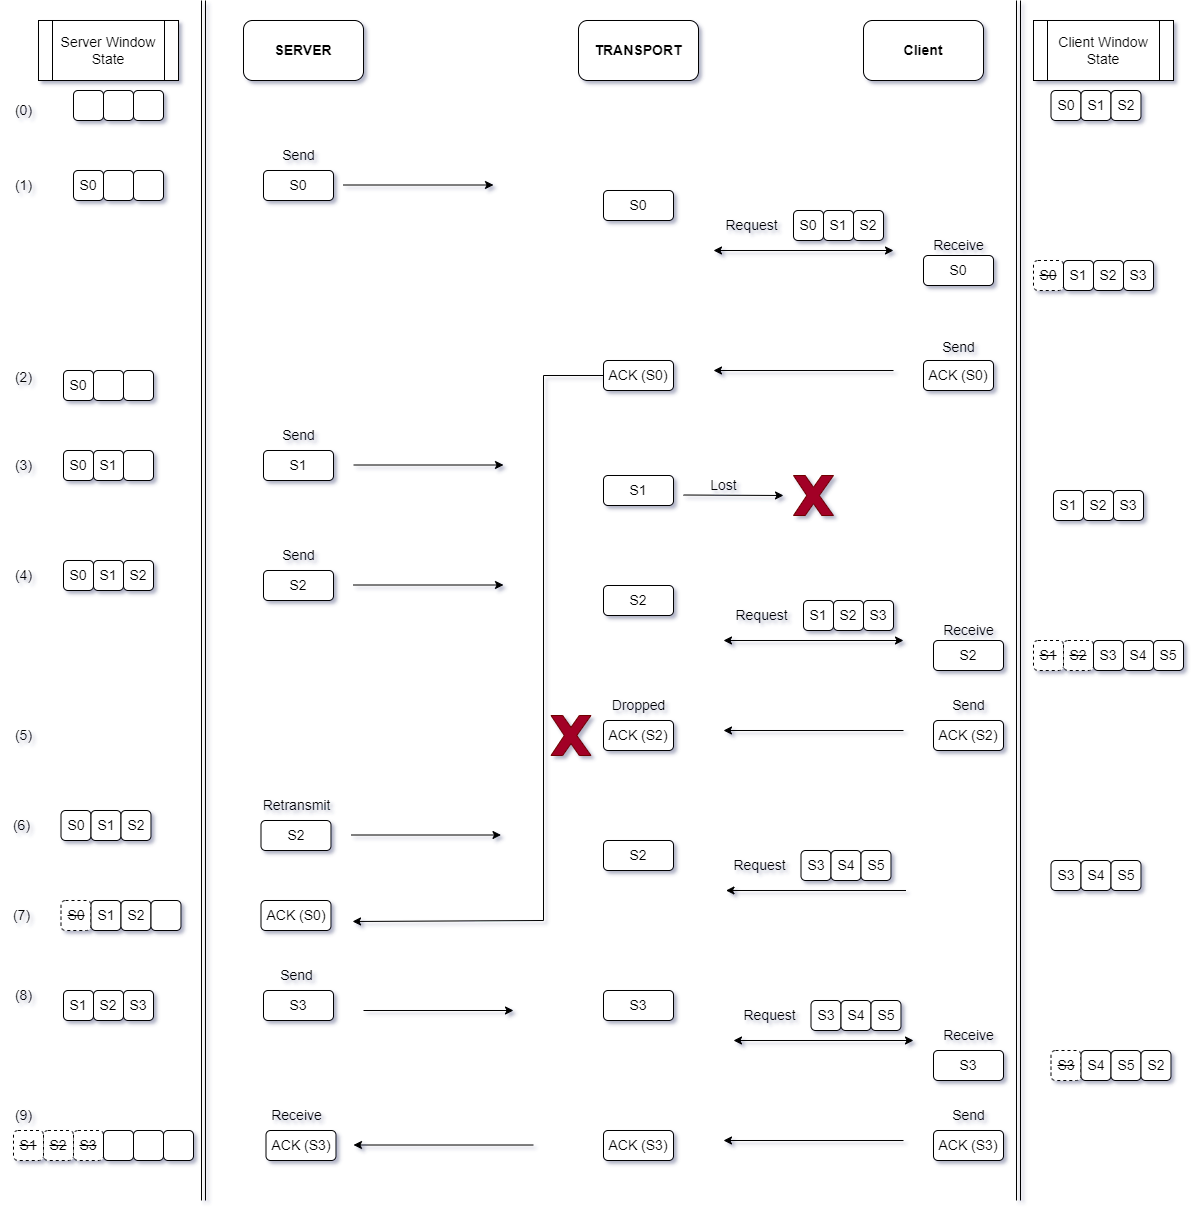
\includegraphics[width= 150mm]{./images/Window_scenarios.drawio.png}
\caption{Scenarios for client and server window}
\end{figure}

\subsection{Scenarios}

\begin{enumerate} [start=0]
    \item Initialize Window
    \begin{enumerate}
        \item Server creates a window of size 3 with empty slots
            \subsubitem Server Window: (null, null, null)
        \item Client also creates a window of size 3 and fills Bundle IDs (S0, S1, S2)
            \subsubitem Client Window: (S0, S1, S2)
    \end{enumerate}
    
    \item Server tries to send S0 \textbf{(Successful Delivery)}
    \begin{enumerate}
        \item Server checks if the window is full, as it is not, it adds S0 to the window and sends S0 to the respective transport
            \subsubitem Server Window: (S0, null, null)
        \item Client requests all bundle IDs in its window (S0, S1, S2) from the transport. The transport only sends S0 as it does not have S1 and S2. On receiving S0, the client window is moved ahead by 1 (as S0 was in position 1 in the window).
            \subsubitem Client Window: (S0, S1, S2) → (S1, S2, S3)
    \end{enumerate}
    
    \item Client tries to send ACK for S0 \textbf{(Out of Order ACK)}
    \begin{enumerate}
        \item Client sends an ACK for the last received bundle ID (S0)
        \item Server does not receive anything at time 2, therefore does nothing.
    \end{enumerate}
    
    \item Server tries to send S1 \textbf{(Bundle Lost)}
    \begin{enumerate}
        \item Server checks if the window is full, as it is not, it adds S1 to the window and sends S1 to the respective transport
            \subitem Server Window: (S0, S1, null)
        \item This is lost and therefore does not get to the client
        \item Client does not receive anything at time 3, therefore does nothing
    \end{enumerate}

    \item Server tries to send S2 \textbf{(Successful Delivery)}
    \begin{enumerate}
        \item Server checks if the window is full, as it is not, it adds S1 to the window and sends S1 to the respective transport
            \subitem Server Window: (S0, S1, S2)
        \item Client requests all bundle IDs in its window (S1, S2, S3) from the transport. The transport only sends S2 as it does not have S1 and S3. On receiving S2, the client window is moved ahead by 2(as S2 was in position 2 in the window).
            \subitem Client Window: (S1, S2, S3) →  (S3, S4, S5)
    \end{enumerate}
    
    \item Client tries to send ACK for S2 \textbf{(Lost/Dropped ACK)}
    \begin{enumerate}
        \item Client sends an ACK for the last received bundle ID (S2)
        \item This is dropped by the transport and does not get to the server
        \item Server does not receive anything at time 5, therefore does nothing
    \end{enumerate}
    
    \item Server tries to send S3 \textbf{(Retransmission)}
    \begin{enumerate}
        \item Server checks if the window is full, it is. It cannot send the new bundle (S3).
        \item It now retransmits the last bundle in the window (S2)
        \item Client requests all bundle IDs in its window (S3, S4, S5) from the transport. The transport only has S2 for the client and so does not send anything to the client
        \item Client does not receive anything at time 6, therefore does nothing
    \end{enumerate}

    \item Server receives ACK \textbf{(Out of order ACK)}
    \begin{enumerate}
        \item Server now receives the ACK sent at time 2 by the client. The ACK received is for Bundle ID S0, the server can now move its window ahead by 1 (as S0 was the first ID in the bundle).
            \subitem Server Window: (S0, S1, S2) →  (S1, S2, null)
    \end{enumerate}

    \item Server tries send S3 again \textbf{(Post retransmission)}
    \begin{enumerate}
        \item Server can now send the bundle S3 as the window is not full after processing the ACK. It adds S3 to the window and sends it to the respective transport
            \subitem Server Window: (S1, S2, null) → (S1, S2, S3)
        \item Client requests all bundle IDs in its window (S3, S4, S5)) from the transport. The transport only sends S3 as it does not have S4 and S5. On receiving S3, the client window is moved ahead by 1(as S3 was in position 1 in the window).
            \subitem Client Window: (S3, S4, S5) → (S4, S5, S6)
    \end{enumerate}

    \item Client tries to send ACK  \textbf{(Successful Delivery)}
    \begin{enumerate}
        \item Client sends an ACK for the last received bundle (S3)
        \item Server receives the ACK bundle and moves its window by 3 (as S3 is in position 3 in the window).
            \subitem Server Window: (S1, S2, null) → (null, null, null)
    \end{enumerate}
\end{enumerate}

\section{Routing}

\begin{figure}[ht!]
\centering
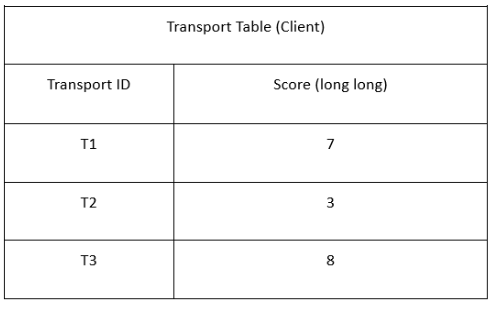
\includegraphics[width= 70mm]{./images/Transport Table.png}
\caption{Transport Table (Client)}
\end{figure}

The Bundle client maintains a table that maps the number of valid bundles (score) received by a transport. A bundle is said to be valid if it is decrypted successfully. This table keeps track of the number of bundles received from all the transports the client comes into contact with. This table is then sent to the Bundle server as part of the meta-data field (see Bundle Header section) to be used in its routing table.

\begin{figure}[ht!]
\centering
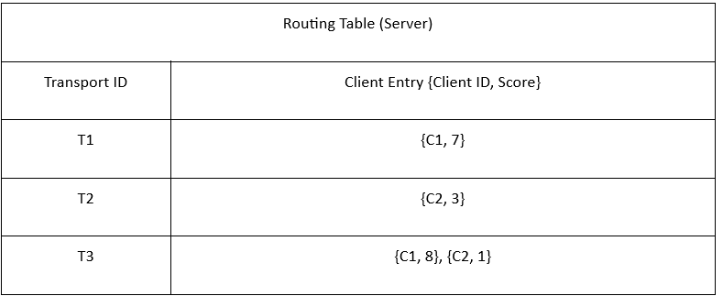
\includegraphics[width= 70mm]{./images/Routing Table.png}
\caption{Routing Table (Server)}
\end{figure}

The Bundle Server maintains a routing table that maps the list of clients that are reachable via a particular Transport. This map is used to determine the following:
\begin{enumerate} [label=(\alph*)]
    \item The list of clients that are reachable via a Transport
    \item The reachability of a client via the transport	
\end{enumerate}

The table shown above describes the routing table as stored on the server. The key is the Transport ID and the values are client entries. Each client entry stores the client ID and a score. The score denotes the number of valid bundles received by the client and is maintained by the client. It is sent to the server as part of the meta-data field of the bundle (See Bundle Header section).

When a bundle is received from a transport, the server checks if the routing table has a record for the current transport. If no record exists, it creates it with the respective Transport ID (TID) and adds a client entry using the client ID (CID) with a score of 0 (as we have not sent anything yet). If a record does exist, it searches for a client entry with the CID of the received bundle in the record. If the client entry is found, it replaces the scores with the score received from the client, otherwise, it creates an entry with the CID and a score of 0. This is repeated for all the transport scores sent by the client.

The score is used to maintain the order of reachability for a particular transport, the list of client entries is therefore sorted in descending order based on the score, to give clients that are known to be reachable, priority over clients that are not as reachable. It is important to note that the priority does NOT mean that the client ID is skipped when sending the list of clients to the Bundle Transmission Module. It simply means that it will be later on the list.
The client entries are NEVER deleted from the routing table as in the worst-case scenario of most transports becoming unavailable, the server can still use a previously connected transport to send data to the client.

The score for a particular client is reset if the received score for the transport remains unchanged for a predetermined number of times. This threshold is denoted as  \textit{reset score} and can be adjusted based on connectivity parameters such as round trip time. \textit{reset score} is initialized to a value of 10, but may be modified dynamically as needed.

\subsection{Special Cases}

\begin{enumerate}
    \item \textbf{Client Moves from one Transport to another/missing:} This can occur if the client or transport no longer meet and a new transport is found.
        \subitem In this case, the client will create a new entry in its table and increment the respective score. On the server side, the new transport will be updated with the client entry. The client entry on the previous transport remains as is. When the same score is reported to the server \textit{reset score} number of times, the score will be reset, resulting in a decreased client priority for the particular transport.
    \item \textbf{Transport only delivers bundles in one direction:} This can occur when the client is only able to receive bundles from the server and all upstream bundles to the server are dropped by the malicious transport.
        \subitem In this case, the client score remains the same as the updates to the server are not sent from that transport. This case is an example of why deleting the client entry from the table could lead to it incorrectly losing connectivity.
    \item \textbf{Client Receives same bundle repeatedly:} This can occur when the server does not get the ACK for a sent bundle, and so retransmits it (Scenario 6 in the Scenario section)
        \subitem In this case, the client has received the bundle before and so does not request the bundle from the transport. The bundle is therefore not sent to the client resulting in the score remaining the same. This case can only be handled at the transport and since it is not a reliable entity we choose the ignore incrementing the score counter in this scenario.
\end{enumerate}


\section{Security}

\subsection{Client ID Generation}

The identity of a client here is its initial public key, this allows other identifiers such as its L2 MAC address from being revealed. As the public key of the client will change at each ratchet step (see Diffie-Hellman Ratchet section), the initial public key will be used throughout as the client ID. Changing the CID each time would result in tables that use the CID as the key on the server side being difficult to maintain and storing redundant and obsolete data.

\subsection{Security Module}

Security modules are implemented on the client and server side. An implementation of the double ratchet algorithm is used to exchange encrypted messages based on a shared secret. The shared secret is derived each time a message must be transmitted or received. There are 3 main components here:
\begin{enumerate}
    \item Diffie-Hellman Ratchet
    \item Root Key Generation
    \item Symmetric Key Ratchet
\end{enumerate}

\subsubsection{Diffie-Helman Ratchet}

\begin{figure}[ht!]
\centering
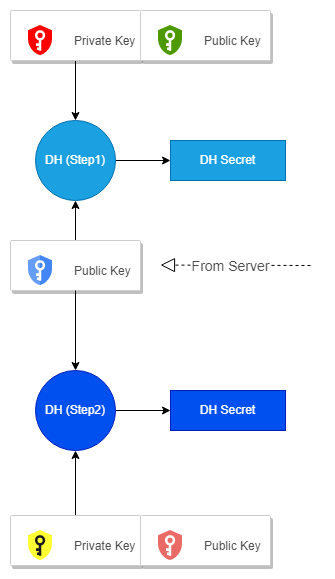
\includegraphics[width= 50mm]{./images/security_overview1-Diffie-Hellman Ratchet.png}
\caption{Diffie-Hellman Ratchet}
\end{figure}

The Diffie-Hellman (DH) ratchet as the name suggests uses the Diffie-Hellman algorithm to generate a shared secret. The Bundle client and server generate a public/private key pair. Initially, the public key of the server is hardcoded into the client allowing it to initiate communication, after which the public key of the sender will be sent to the receiver along with the bundle.

When a new public key is received, a ratchet step is performed; the receiver as shown in Figure 7 uses its current private key along with the received private key to generate a DH Secret to match the secret generated by the sender (DH step 1 of Figure 7). The receiver then generates a new public/private key pair and calculates a new DH secret (DH step 2 of Figure 7). This cycle is repeated every time a new public key is received.
If any of the private keys in this exchange is compromised, it is isolated from all other secrets that are generated as each message will have a new secret. This is called forward secrecy wherein an intermediate key if compromised cannot be used to compromise later messages. Similarly, backward secrecy is also maintained as we cannot use the current key to compromise previous messages.

The DH secret that is generated is used as an input to a Key Derivation Function (KDF) to derive a sending and receiving chain key. The details of how the chain keys are derived will be explained in later sections, however, the use of the DH secret is as follows.

The DH secret generated in step 1 is used to generate a sending key on the client when it initiates communication. The server on its end will also generate a DH secret using its private key along with the client’s public key that it receives. The derived secret is the same as it is generated using the DH exchange. This shared secret is passed to a KDF to derive a receiving and sending chain key on the client and server respectively to generate the same symmetric encryption key.

\subsubsection{Root Key Generation}
The Root Key is generated using a pre-key bundle the first time, subsequent generations of the root key are derived using a Key Derivation Function (KDF).

\begin{figure}[ht!]
\centering
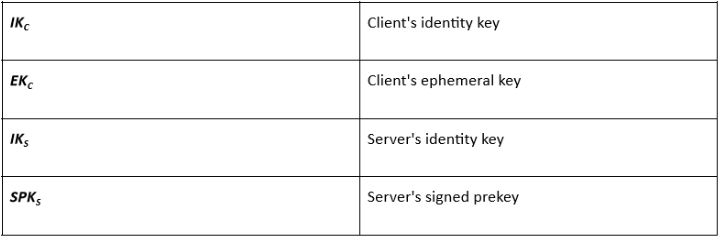
\includegraphics[width= 70mm]{./images/Key Table.png}
\caption{Key Table}
\end{figure}

\subsubsection{Initial Root Key Generation}
The root key is calculated using 3 Diffie-Hellman key exchanges as follows:
\begin{enumerate}
    \item DH1 = IK\textsubscript{C}   +  SPK\textsubscript{S}
    \item DH2 = EK\textsubscript{C}   +  IK\textsubscript{S}
    \item DH3 = EK\textsubscript{C}   +  SPK\textsubscript{S}
\end{enumerate}

The resulting DH secrets namely DH1, DH2 and DH3 are passed to a KDF, which returns the root key.
Root Key = KDF(DH1, DH2, DH3)
This is used as the initial root key.

\subsubsection{Subsequent Root Key Generation}
\begin{figure}[ht!]
\centering
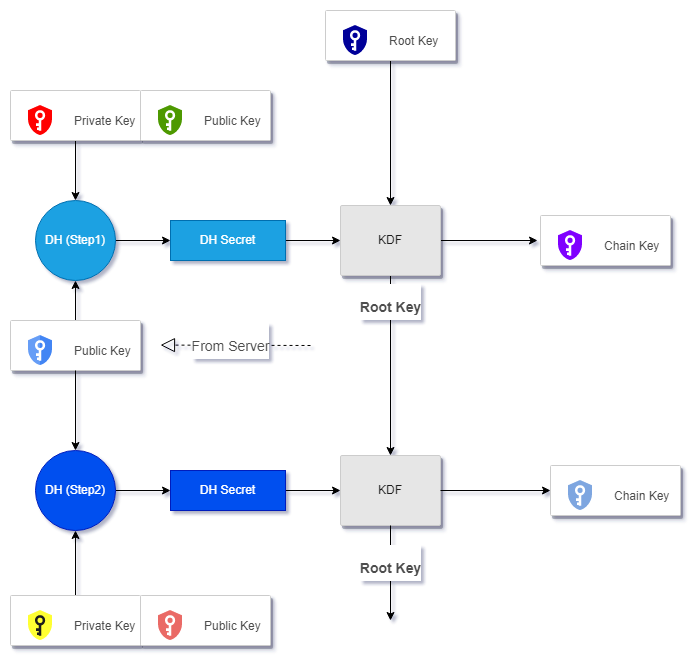
\includegraphics[width= 100mm]{./images/security_overview1-Root Key Generation.png}
\caption{Root Key Generation}
\end{figure}

Once the initial root key is generated, all subsequent root keys are generated by the KDF with the inputs being the previous Root Key and the new Diffie-Hellman Secret as shown in Figure 9. The KDF also generates a Chain key. This is used to generate the sending or receiving chain keys and is described in the next section.

The requirement while selecting a KDF is that it must guarantee all outputs appear random, regardless of the inputs selected. The Hash-based message authentication code (HMAC) and HMAC-based key derivation function (HKDF) constructions, when instantiated with a secure hash algorithm, meet the KDF definition. KDFs therefore, provide forward security as the outputs appear random and have no relation to a previous or later output.

\subsubsection{Symmetric Key Ratchet}
The last ratchet in this algorithm is a symmetric key ratchet. These keys are also generated similarly using a KDF with the root key. The inputs to the KDF here are, the Chain key generated by the previous KDF and a constant value. The KDF provides 2 outputs here as well; a chain key that will be used in the next ratchet step to generate further keys and a message key. The message key is used to encrypt or decrypt the message for the sending and receiving chains respectively. The Message keys can be stored to be used later on when handling out-of-order messages as they are not used to generate new keys. Figure 10 illustrates the entire flow that is triggered when a new public key is received from the server. 

\begin{figure}[ht!]
\centering
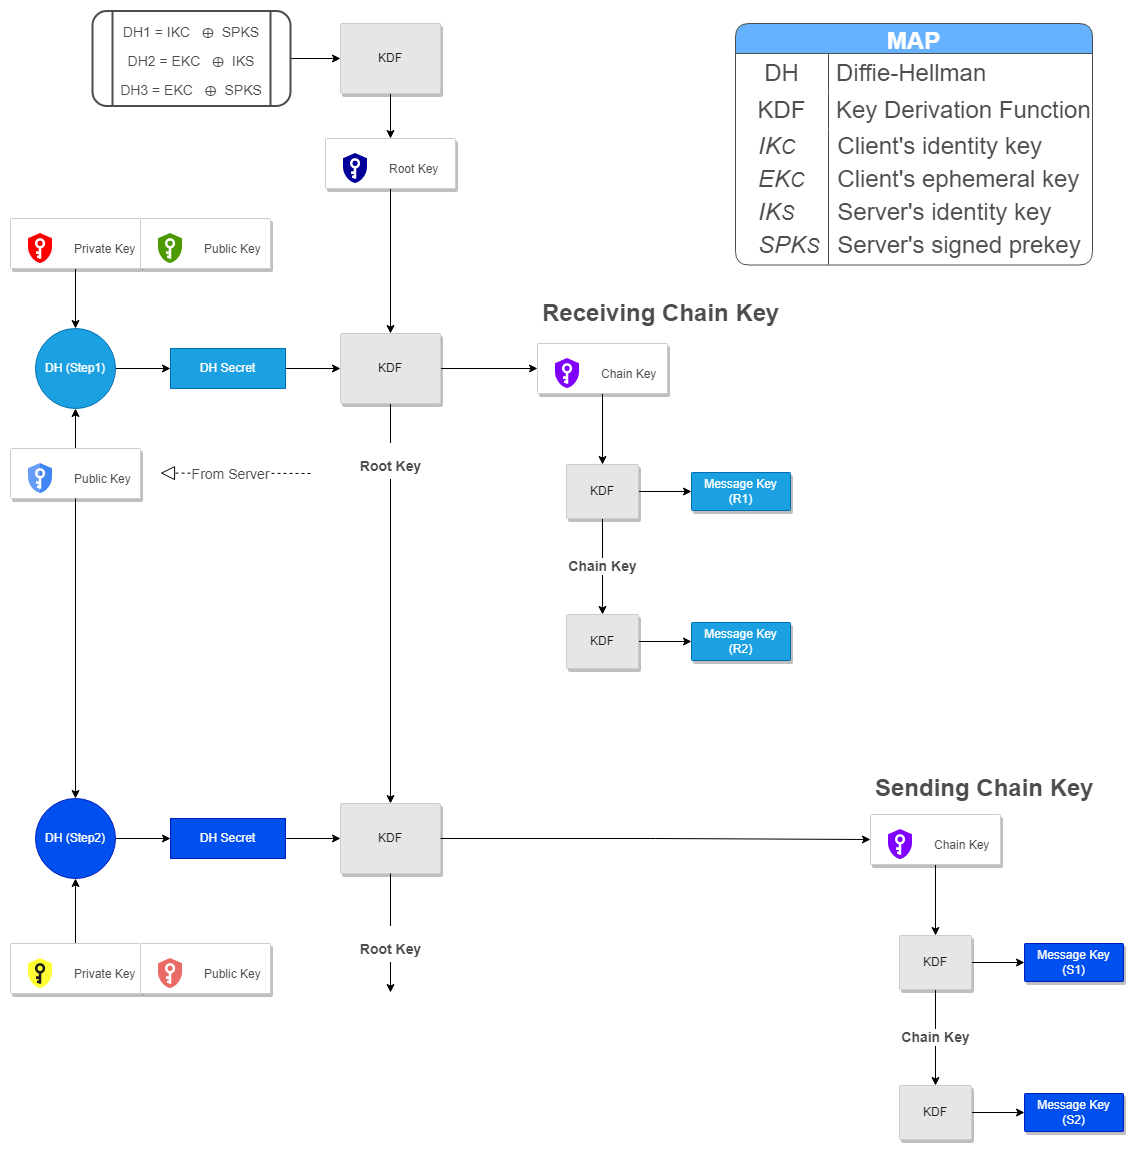
\includegraphics[width= 150mm]{./images/security_overview1-Overview.png}
\caption{Security Overview}
\end{figure}

\section{Bundle Format}
\begin{figure}[ht!]
\centering
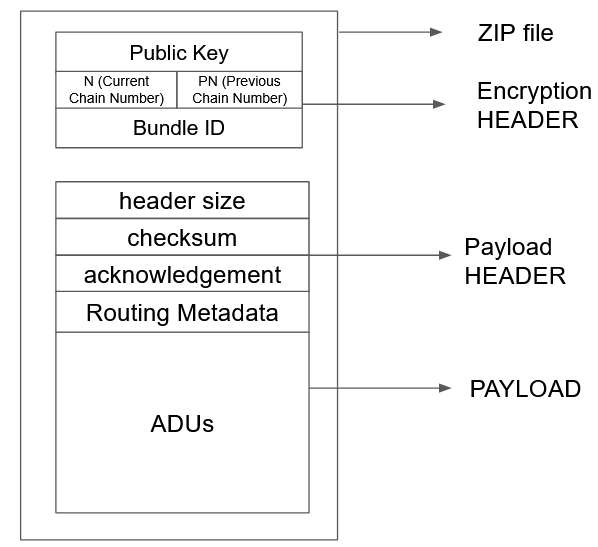
\includegraphics[width= 70mm]{./images/Bundle Header.png}
\caption{Bundle Format}
\end{figure}

The Bundle has a collection of fields that contains identifying and processing information along with the application data. The fields are as follows:
\begin{enumerate}
    \item \textbf{Encryption Header:} This field consists of the parameters required to decrypt the bundle including the Public key of the sender along with the current (N) and previous chain number (PN)
    \item \textbf{Bundle ID:} The generated bundle ID is stored here (This is the encrypted Bundle ID).
    \item \textbf{Payload Header:} This field includes the data required to parse the payload's header such as the header size, checksum, acknowledgments to be sent i.e., the Bundle ID to be acknowledged and the routing metadata. The routing metadata field is filled only by the Bundle client and stores the client's Transport table as described in Routing Section.
    \item \textbf{ADUs:} This field stores all of the application data units (ADUs) that need to be sent.
\end{enumerate}

The payload and its associated header are encrypted using the key and ratchet specified in the encryption header. This encrypted data, along with the encryption header and bundle ID, are then compressed and packaged into a zip file.

\section{Double Ratchet Scenarios}
\begin{figure}[ht!]
\centering
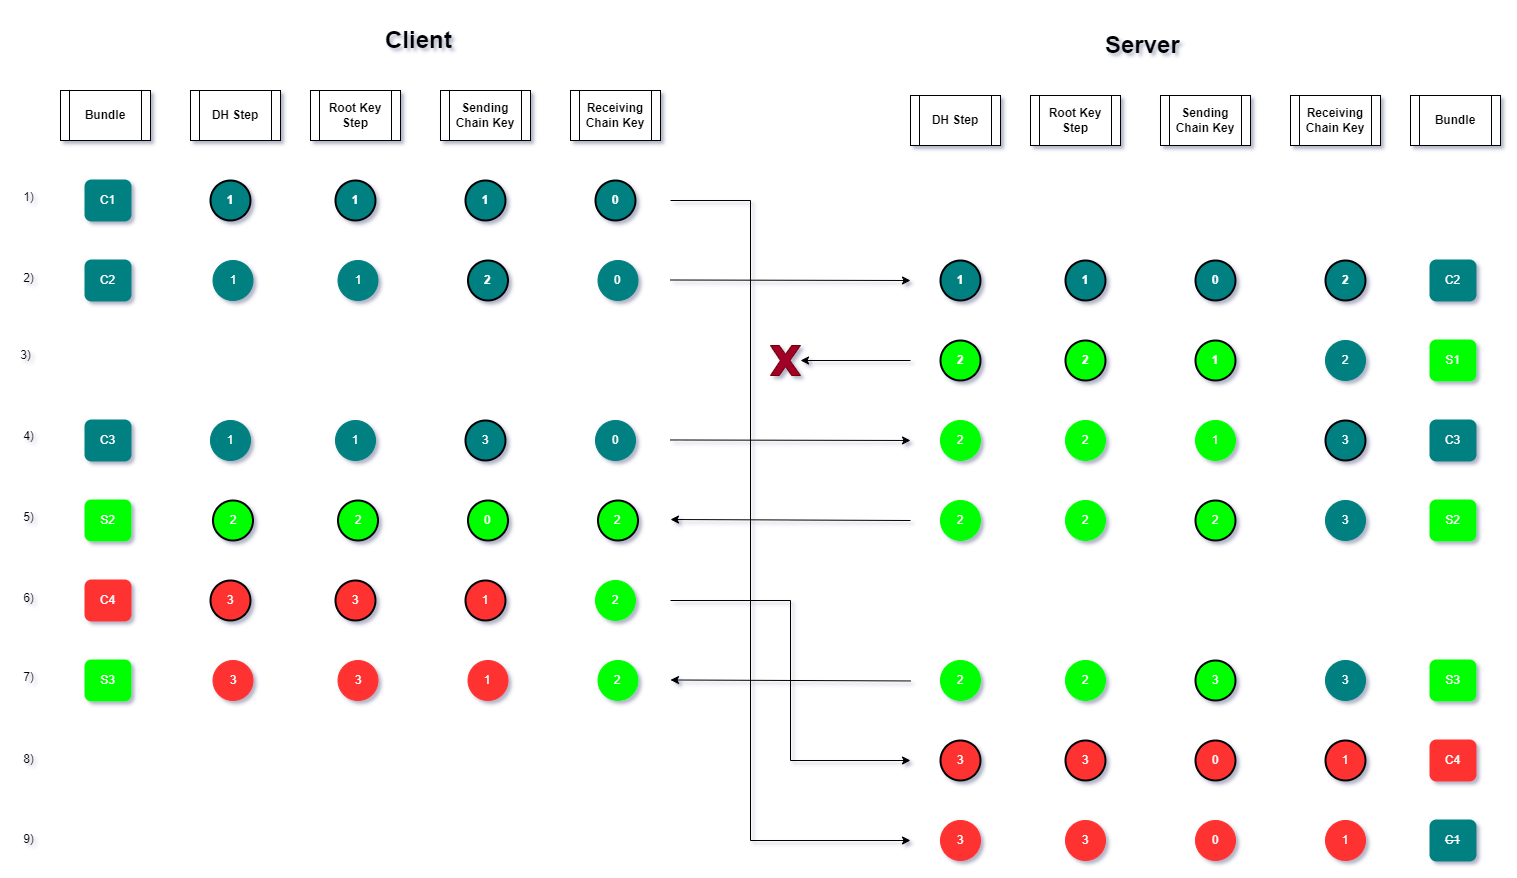
\includegraphics[width= 150mm]{./images/Ratchet Scenarios.png}
\caption{Ratchet Scenarios}
\end{figure}

The following scenarios describe the ratchet steps that take place to create encryption/decryption keys. Each bundle also consists of the N and PN values that describe the current and previous chain numbers and are used to synchronize the chains at either end.

\begin{enumerate}
    \item Client tries to send C1 \textbf{(Out of Order)}
    \begin{enumerate}
        \item Client sends bundle C1 with its first DH and sending chain key ratchet step
        \item Server does not receive it at time 1, therefore does nothing
    \end{enumerate}
    
    \item Client tries to send C2 \textbf{(Server Ratchet Initialization)}
    \begin{enumerate}
        \item Client moves its sending ratchet to 2 with all other ratchets remaining the same
        \item Server receives the bundle with a new public key, initializes its ratchets with the key and moves its receiving ratchet to the N value provided (2). The sending ratchet stays the same.
    \end{enumerate}

    \item Server tires to send S1 \textbf{(New Ratchet Step)}
    \begin{enumerate}
        \item The server moves its DH ratchet to 2, resulting in resetting the sending ratchet. It is now incremented and a key is generated using the new DH secret. The receiving ratchet is not reset as it has not received a new public key from the client.
        \item The client does not receive the bundle and therefore does nothing
    \end{enumerate}
    
    \item Client tries to send C3 \textbf{(Out of Order Delivery)}
    \begin{enumerate}
        \item Client moves its sending ratchet to 3 with all other ratchets remaining the same
        \item Server receives the bundle with the previous key, the receiving chain is, therefore, incremented to the N value of 3. All other ratchets remain the same.
    \end{enumerate}

    \item Server tries to send S2 \textbf{(Reset Client Ratchets)}
    \begin{enumerate}
        \item Server moves its sending ratchet to 2 with all the other ratchets remaining the same
        \item Client receives the bundle with the new public key and resets all of its ratchets. It then moves its receiving ratchet to the N value of 2.
    \end{enumerate}

    \item Client tries to send C4 \textbf{(Increment Client DH Ratchet)}
    \begin{enumerate}
        \item Client now increments its DH ratchet, resetting its sending key ratchet as well. The sending ratchet is then incremented. The receiving ratchet stays the same.
        \item Server does not receive anything and therefore does nothing
    \end{enumerate}

    \item Server tries to send S3 \textbf{(Successful Delivery)}
    \begin{enumerate}
        \item Server moves its sending ratchet to 3 with all the other ratchets remaining the same
        \item Client receives the bundle with the previous key, the receiving chain is, therefore, incremented to the N value of 3. All other ratchets remain the same.
    \end{enumerate}

    \item Server receives C4 \textbf{(Out of Order Delivery)}
    \begin{enumerate}
        \item Server receives bundle C4, it has a new public key, a new DH step is taken and all of the ratchets are reset. The receiving chain is then set to the N value of 1.
    \end{enumerate}

    \item Server receives C1 \textbf{(Out of Order Delivery)}
    \begin{enumerate}
        \item Server receives an older message C1, this is ignored as newer messages have already been received and the window is moved ahead (See window section)
    \end{enumerate}
\end{enumerate}

